\chapter{PROPOSTA}
\label{chap:proposta}

Este capítulo apresenta o projeto detalhado, os requisitos e a arquitetura da solução \nome\ (\textit{Slice-aware Polynomial Key-based Architecture}), concebida para abordar as limitações de escalabilidade, inflexibilidade do plano de dados e isolamento de Qualidade de Serviço (QoS) no fatiamento de redes cientes de caminho descritas no Capítulo~\ref{chap:introducao}.

A proposta unifica o roteamento na origem sem estados no núcleo --- baseado em Sistemas de Numeração de Resíduos (\textit{Residue Number System} -- RNS) e aritmética polinomial sobre o corpo finito de Galois $GF(2)$ --- com mecanismos programáveis de enfileiramento e escalonamento de pacotes. Ao delegar a classificação e a codificação das políticas de rede exclusivamente aos nós de borda, o \nome\ permite que os comutadores de núcleo executem o encaminhamento e a seleção de filas de prioridade em taxa de linha (\textit{line-rate}) sem a necessidade de manutenção de tabelas de estado por fluxo ou por fatia.

% ==============================================================================
\section{Levantamento de Requisitos}
\label{sec:requisitos}

Para suportar o fatiamento de redes (\textit{Network Slicing}) em redes cientes de caminho --- nas quais coexistem fluxos e aplicações heterogêneas com requisitos antagônicos de vazão, atraso e confiabilidade ---, a arquitetura de transporte deve garantir isolamento lógico e de desempenho sem comprometer a escalabilidade do plano de controle. Com base na análise da literatura e nas lacunas identificadas nos trabalhos relacionados, foram estabelecidos os requisitos funcionais (RF) e não funcionais (RNF) que norteiam o projeto do \nome, sintetizados nas Tabelas~\ref{tab:req_funcionais} e~\ref{tab:req_nao_funcionais}.

\begin{table}[htb]
    \centering
    \caption{Requisitos Funcionais da arquitetura \nome.}
    \label{tab:req_funcionais}
    \begin{tabular}{p{1.8cm} p{12.5cm}}
        \hline
        \textbf{Código} & \textbf{Descrição do Requisito Funcional} \\
        \hline
        \textbf{RF01} & \textbf{Codificação unificada de rota e QoS:} Codificar, em um único rótulo de comprimento fixo inserido na borda da rede, tanto a trajetória explícita quanto a política de enfileiramento para cada salto do caminho. \\
        \textbf{RF02} & \textbf{Encaminhamento e seleção de fila sem estados no núcleo:} Permitir que os comutadores de núcleo determinem simultaneamente a interface de egresso e o identificador da fila de serviço por meio de operações aritméticas locais, eliminando tabelas de roteamento e de QoS por fatia no núcleo. \\
        \textbf{RF03} & \textbf{Classificação flexível e mapeamento de fatias na borda:} Classificar os fluxos ingressantes a partir de qualquer campo de cabeçalho ou metadado de serviço (tais como marcações DSCP, etiquetas VLAN/PCP, rótulos MPLS TC, prefixos IP, portas L4 ou identificadores de fatia) e encapsulá-los com o respectivo rótulo de rota e QoS. \\
        \textbf{RF04} & \textbf{Isolamento de recursos via escalonamento ponderado:} Viabilizar garantias mínimas de largura de banda e priorização entre fatias concorrentes ao direcionar os pacotes para filas previamente configuradas sob políticas de escalonamento ponderado nas interfaces de saída, evitando a inanição (\textit{starvation}) de filas de menor prioridade. \\
        \textbf{RF05} & \textbf{Reconfiguração ágil de rotas e políticas:} Viabilizar a migração dinâmica de caminhos e a alteração de classes de serviço de uma fatia em tempo de execução mediante a atualização exclusiva das regras nos nós de borda. \\
        \hline
    \end{tabular}
    \fonte{Elaborado pelo autor (2026).}
\end{table}

\begin{table}[htb]
    \centering
    \caption{Requisitos Não Funcionais da arquitetura \nome.}
    \label{tab:req_nao_funcionais}
    \begin{tabular}{p{1.8cm} p{12.5cm}}
        \hline
        \textbf{Código} & \textbf{Descrição do Requisito Não Funcional} \\
        \hline
        \textbf{RNF01} & \textbf{Processamento em taxa de linha (\textit{line-rate}):} As operações de decodificação de rota e fila no plano de dados devem explorar primitivas nativas de hardware ou do núcleo do sistema operacional (como unidades de CRC e ganchos eBPF/XDP), garantindo latência determinística e alto desempenho. \\
        \textbf{RNF02} & \textbf{Baixa sobrecarga no plano de controle:} Eliminar a necessidade de sinalização e atualização coordenada em múltiplos dispositivos intermediários durante a criação, modificação ou remoção de fatias de rede. \\
        \textbf{RNF03} & \textbf{Imutabilidade e compacidade de cabeçalho:} Manter o cabeçalho de transporte com tamanho fixo e inalterado ao longo de todo o domínio de núcleo, evitando operações de reescrita ou remoção de rótulos salto a salto. \\
        \textbf{RNF04} & \textbf{Portabilidade arquitetural:} Permitir a implantação do plano de dados tanto em ambientes de emulação programável (e.g., P4/BMv2) quanto em planos de dados de alto desempenho baseados em hardware programável (e.g., Intel Tofino) ou no \textit{kernel} Linux (eBPF/XDP). \\
        \hline
    \end{tabular}
    \fonte{Elaborado pelo autor (2026).}
\end{table}

% ==============================================================================
\section{Arquitetura do Protocolo SPolKA}
\label{sec:arquitetura_spolka}

O protocolo \nome\ estende a arquitetura de roteamento na origem PolKA (\textit{Polynomial Key-based Architecture}) \cite{dominicini2020} ao incorporar, de forma nativa e sem estados no núcleo, o endereçamento de filas de serviço para o fatiamento em redes cientes de caminho. Enquanto abordagens tradicionais de roteamento na origem baseadas em empilhamento de rótulos exigem que cada salto remova ou atualize o cabeçalho --- incorrendo em sobrecarga crescente proporcional ao diâmetro da rede ---, o \nome\ codifica toda a trajetória e as respectivas políticas de QoS em um único identificador compacto e imutável ao longo do núcleo.

Estruturalmente, a arquitetura do \nome\ organiza-se em três camadas funcionais desacopladas, conforme ilustrado na Figura~\ref{fig:spolka_camadas}, seguindo o paradigma de Redes Definidas por Software (SDN) com planos de dados programáveis:
\begin{itemize}
    \item \textbf{Camada de Serviço:} Compreende as aplicações finais, funções de rede virtuais e sistemas de orquestração de fatias em redes cientes de caminho que demandam garantias específicas de Acordo de Nível de Serviço (SLA), expressas por meio de classes de tráfego diferenciadas ou identificadores de fatia.
    \item \textbf{Camada de Controle e Orquestração:} Centraliza a inteligência da rede e subdivide-se em quatro módulos lógicos: (i) \textit{Conhecimento da topologia}, responsável por mapear a infraestrutura física e monitorar o estado dos enlaces; (ii) \textit{Cálculo de caminhos}, que seleciona a sequência de saltos adequada aos requisitos de QoS de cada fatia; (iii) \textit{Geração polinomial do \routeID\ (CRT)}, encarregado de atribuir identificadores únicos aos nós e sintetizar os rótulos de rota e fila via Teorema Chinês dos Restos; e (iv) \textit{Políticas de filas (\qID\ e pesos WDRR)}, que define as configurações dos escalonadores e instala proativamente as regras de classificação nas tabelas dos comutadores de borda.
    \item \textbf{Camada de Infraestrutura Física (Plano de Dados):} Constituída por elementos de encaminhamento programáveis (como dispositivos habilitados para P4 ou \textit{hosts}/roteadores executando eBPF/XDP) divididos logicamente entre nós de borda --- que executam a classificação, o encapsulamento e o desencapsulamento dos rótulos --- e nós de núcleo, que operam de forma totalmente \textit{stateless} no encaminhamento e na seleção das filas dos pacotes.
\end{itemize}

\begin{figure}[!htb]
    \centering
    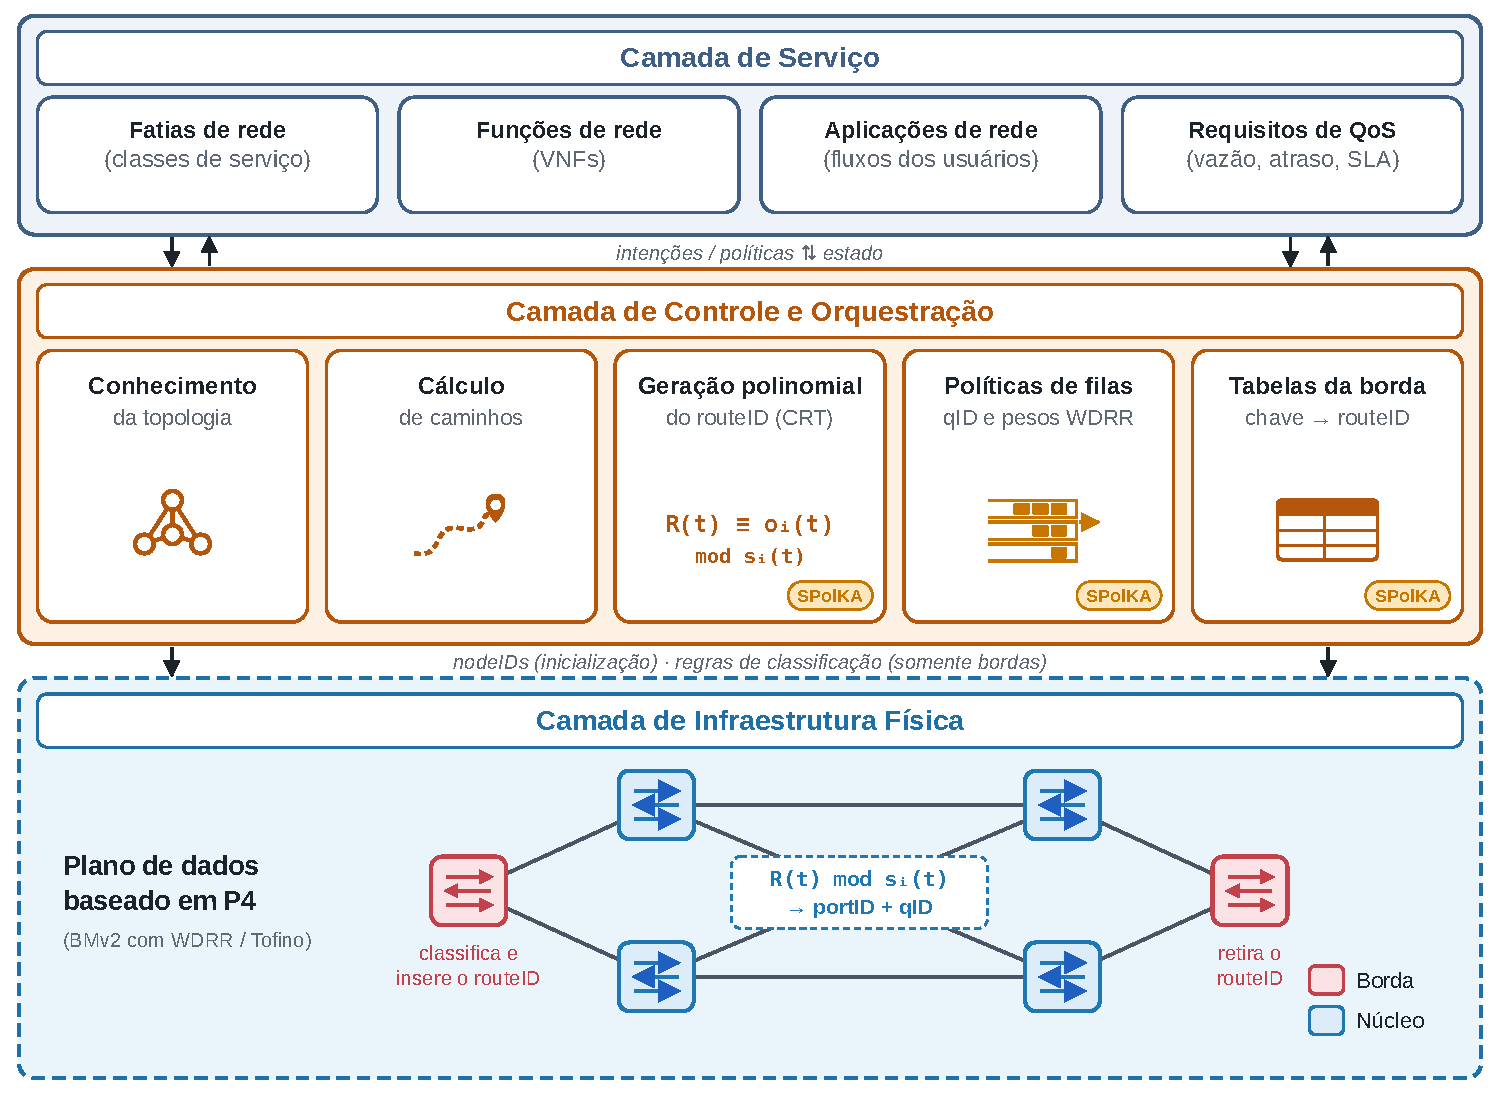
\includegraphics[width=\textwidth]{figuras/fig_arq_camadas_spolka.pdf}
    \captionsetup{justification=centering}
    \caption{Arquitetura em camadas do \nome\ e interação entre serviço, controle e plano de dados.}
    \label{fig:spolka_camadas}
\end{figure}

\subsection{Formulação Matemática e Codificação em $GF(2)$}
\label{subsec:formulacao_matematica}

O funcionamento operacional da arquitetura divide-se logicamente em três etapas principais: (i) a atribuição de identificadores e o cálculo do rótulo no Plano de Controle; (ii) a classificação e o encapsulamento na borda de ingresso; e (iii) o encaminhamento e a seleção de fila sem estados nos comutadores de núcleo.

Para formalizar o processo de codificação, considere um fluxo de tráfego de uma fatia que deve atravessar um caminho selecionado composto por $N$ nós de núcleo. Na fase de inicialização da topologia, o Controlador atribui a cada comutador de núcleo um identificador único representado por um polinômio irredutível $s_i(t)$ sobre o corpo finito de Galois $GF(2)$, formando o conjunto ordenado $S = \{s_1(t), s_2(t), \ldots, s_N(t)\}$ dos \nodeIDs\ ao longo do trajeto. Para garantir a unicidade da solução matemática, os polinômios pertencentes ao conjunto $S$ devem ser necessariamente coprimos entre si.

Simultaneamente, o Controlador define as ações de encaminhamento e priorização que cada nó intermediário deverá executar. Para cada salto $i \in \{1, 2, \ldots, N\}$, estabelece-se um polinômio de saída $o_i(t)$, pertencente ao conjunto $O = \{o_1(t), o_2(t), \ldots, o_N(t)\}$. Diferentemente da abordagem original do PolKA, na qual o resíduo codifica exclusivamente a interface de egresso, no \nome\ o polinômio $o_i(t)$ resulta da concatenação binária entre o identificador da porta física de saída (\portID) e o identificador da fila de serviço (\qID) atribuída ao fluxo naquele nó. Para que a recuperação dessa informação ocorra sem ambiguidades na operação de módulo, cada par de polinômios deve satisfazer estritamente a restrição de grau dada por $\text{grau}(s_i) > \text{grau}(o_i)$.

De posse dos conjuntos $S$ e $O$, o Controlador sintetiza o identificador global da fatia e da rota, denominado \routeID\ e representado pelo polinômio $R(t)$, por meio da aplicação do Teorema Chinês dos Restos (CRT) polinomial \cite{Shoup:2009, dominicini2020}. O polinômio $R(t)$ é calculado de modo a satisfazer simultaneamente o seguinte sistema de congruências lineares em $GF(2)$:

\begin{equation}
\label{eq:crt_spolka}
R(t) \equiv o_i(t) \pmod{s_i(t)}, \quad \forall i \in \{1, 2, \ldots, N\}
\end{equation}

Uma vez computado o \routeID, o Controlador traduz a política de engenharia de tráfego instalando regras de correspondência (\textit{match-action}) exclusivamente nos comutadores de borda da rede. No nó de ingresso, o tráfego entrante pode ser classificado a partir de qualquer campo de cabeçalho ou metadado de serviço --- tais como marcações DiffServ (DSCP), etiquetas VLAN/PCP, rótulos MPLS TC, prefixos IP, portas da camada de transporte ou identificadores de fatia --- e associado ao respectivo \routeID, que é então inserido no cabeçalho do pacote. Graças às propriedades aritméticas dos polinômios sobre $GF(2)$, o rótulo $R(t)$ permanece inalterado durante todo o percurso pelo domínio de transporte, sendo removido apenas pelo comutador de egresso antes da entrega ao destino final.

No plano de dados dos comutadores de núcleo, o encaminhamento opera de maneira totalmente desprovida de estados de fluxo (\textit{stateless}), eliminando a necessidade de tabelas de roteamento ou de manutenção de contexto por fatia. Ao receber um pacote encapsulado, cada nó de núcleo $i$ extrai simultaneamente a porta de destino e a fila de escalonamento calculando o resto da divisão polinomial (operação de módulo) entre o \routeID\ contido no cabeçalho e o seu próprio \nodeID\ localmente armazenado:

\begin{equation}
\label{eq:mod_spolka}
o_i(t) = \langle R(t) \rangle_{s_i(t)} = R(t) \bmod s_i(t)
\end{equation}

Em termos de implementação em hardware programável ou planos de dados acelerados (como P4 e eBPF), essa operação aritmética em $GF(2)$ equivale diretamente ao cálculo de verificação cíclica de redundância (CRC), permitindo sua execução em taxa de linha (\textit{line-rate}) com latência determinística. O valor binário resultante $o_i(t)$ é então particionado por meio de operações simples de deslocamento e mascaramento de bits (\textit{bit-slicing}): os bits mais significativos determinam o \portID\ para o qual o pacote deve ser comutado, enquanto os bits menos significativos especificam o \qID\ no gerenciador de tráfego (\textit{Traffic Manager}) da interface de saída. Ao direcionar os fluxos para filas previamente configuradas sob políticas de escalonamento ponderado nos nós intermediários, o \nome\ viabiliza o isolamento de largura de banda entre fatias concorrentes sem manter estado no núcleo.

\begin{figure}[!htb]
    \centering
    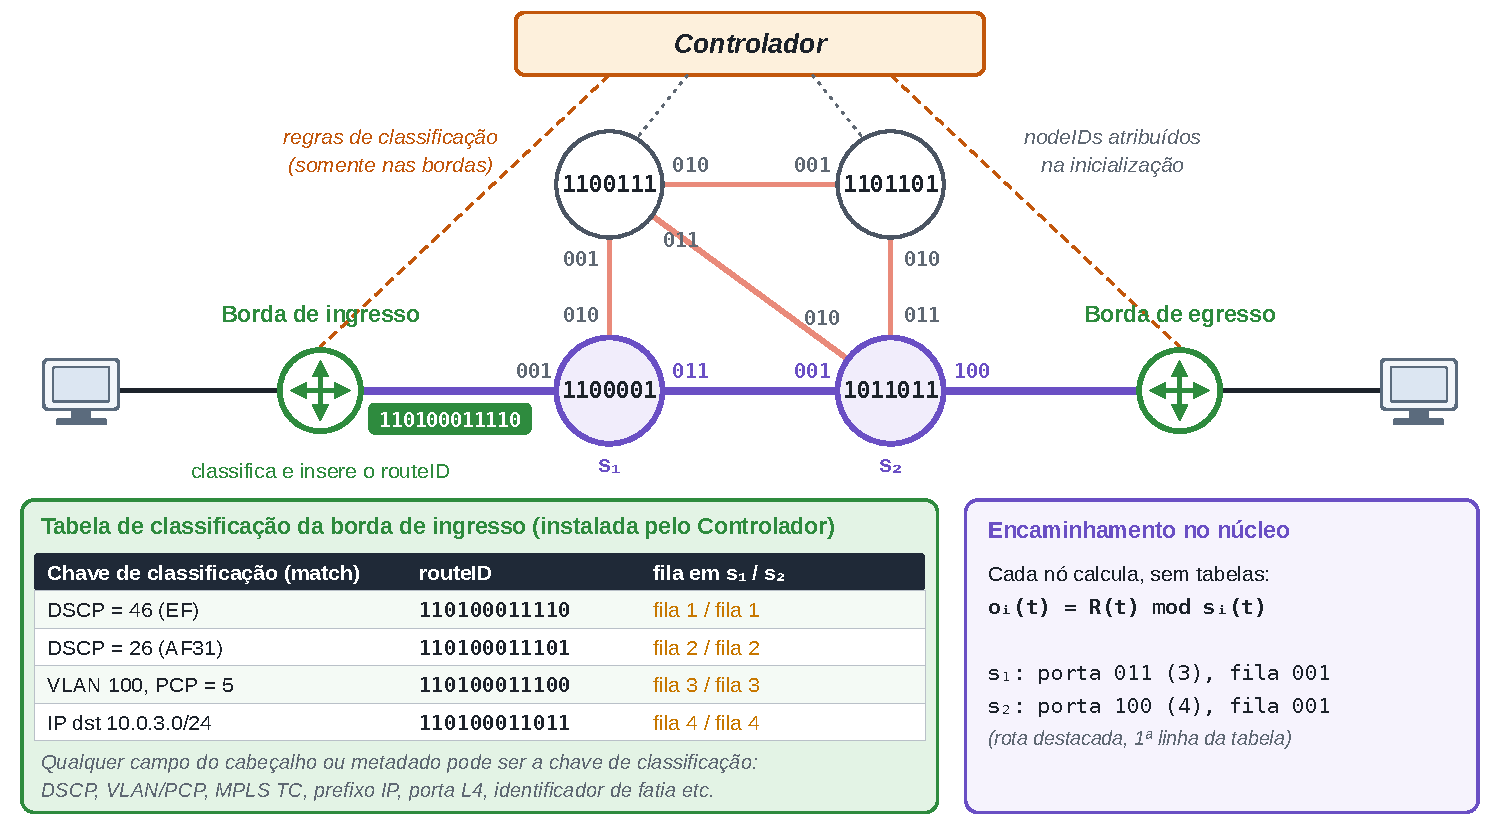
\includegraphics[width=\textwidth]{figuras/fig_arq1_visao_geral.pdf}
    \captionsetup{justification=centering}
    \caption{Visão geral da arquitetura \nome\ e tabela de classificação flexível na borda de ingresso.}
    \label{fig:spolka_visao_geral}
\end{figure}

A Figura~\ref{fig:spolka_visao_geral} apresenta a visão geral da arquitetura \nome\ e a operação do plano de dados na borda em uma topologia ciente de caminho cujos identificadores atribuídos pelo Controlador incluem os polinômios $s_1(t) = t^6 + t^5 + 1$ (representado em binário por $1100001$) e $s_2(t) = t^6 + t^4 + t^3 + t + 1$ ($1011011$). Para estabelecer o caminho $s_1 \rightarrow s_2$ com políticas específicas de enfileiramento em cada salto, o Controlador aplica o CRT polinomial (Equação~\ref{eq:crt_spolka}) e obtém o rótulo $R(t) = 110100011110$, associando-o à respectiva chave de classificação (como $\text{DSCP} = 46$, VLAN ou prefixo IP) na tabela de fluxo da borda de ingresso.

\begin{figure}[!htb]
    \centering
    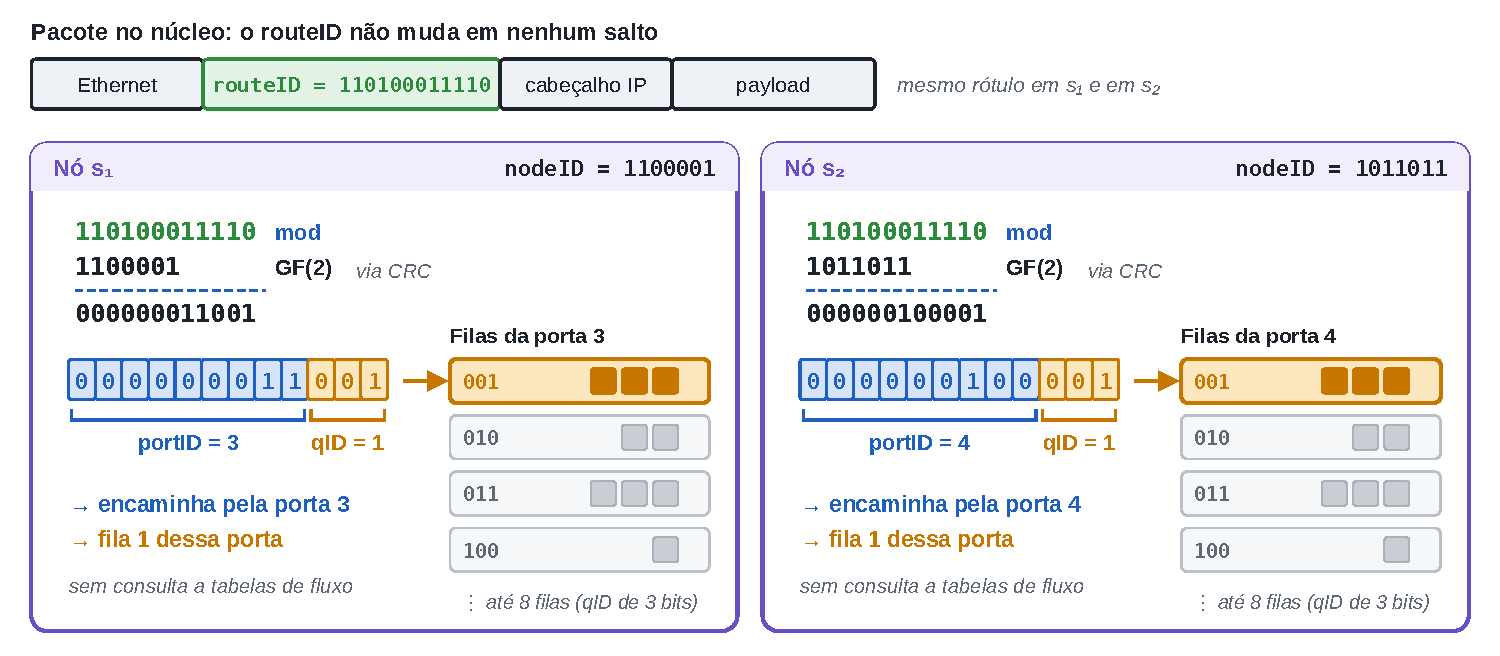
\includegraphics[width=\textwidth]{figuras/fig_arq2_nucleo.pdf}
    \captionsetup{justification=centering}
    \caption{Processamento sem estado (\textit{stateless}) e extração simultânea de porta e fila nos comutadores de núcleo do \nome.}
    \label{fig:spolka_nucleo}
\end{figure}

O detalhamento da operação executada internamente nos nós intermediários é ilustrado na Figura~\ref{fig:spolka_nucleo}. Quando o pacote alcança o primeiro nó de núcleo ($s_1$), o comutador executa a divisão polinomial em $GF(2)$ (via CRC) entre o rótulo imutável $R(t) = 110100011110$ e seu identificador local $s_1(t) = 1100001$ (Equação~\ref{eq:mod_spolka}), extraindo o resto $o_1(t) = 000000011001$. Na decomposição desse resultado, os bits mais significativos (\portID\ $= 3$, ou $011$) instruem o plano de dados a encaminhar o pacote pela porta física 3, ao passo que os bits menos significativos (\qID\ $= 1$, ou $001$) direcionam o pacote à fila 1 daquela interface. De maneira análoga e independente, ao chegar ao nó subsequente ($s_2$), o mesmo rótulo $R(t)$ é dividido por $s_2(t) = 1011011$, resultando em $o_2(t) = 000000100001$, o que determina o encaminhamento pela porta física 4 (\portID\ $= 4$) e o enfileiramento na fila 1 (\qID\ $= 1$), sem qualquer consulta a tabelas de fluxo. Por fim, o switch de borda de egresso remove o cabeçalho do \routeID\ e entrega o pacote original ao destino.

% ==============================================================================
\section{Formato do Cabeçalho e Decodificação no Plano de Dados}
\label{sec:formato_cabecalho}

Para viabilizar a operação independente de protocolo em comutadores programáveis, o cabeçalho do \nome\ é inserido imediatamente após o cabeçalho Ethernet padrão, sendo identificado por um valor específico no campo \textit{EtherType}\footnote{Por se tratar de um protocolo experimental, o identificador de \textit{EtherType} utilizado pelo \nome\ é definido arbitrariamente para fins de prototipação, não possuindo registro formal junto ao IEEE (\textit{Institute of Electrical and Electronics Engineers}). Nos ambientes de experimentação e testes em laboratório deste trabalho, adotou-se o valor \texttt{0x1234}.} que sinaliza aos nós intermediários a presença do rótulo de roteamento na origem. Diferentemente das abordagens baseadas em empilhamento de segmentos, o cabeçalho do \nome\ possui comprimento fixo determinado pelo diâmetro máximo da rede e pelo grau dos polinômios geradores adotados.

Seguindo a análise de escalabilidade do RNS polinomial \cite{dominicini2020}, o tamanho em bits do campo \routeID\ é dado pelo produto entre o número máximo de saltos suportados na topologia ($H_{\max}$) e o grau $r$ dos polinômios irredutíveis utilizados (tipicamente $r = 16$ bits para unidades CRC-16, o que suporta até $4.080$ nós de núcleo distintos). Na arquitetura projetada neste trabalho, adotou-se $H_{\max} = 10$ saltos com polinômios de grau $16$, resultando em um identificador \routeID\ de comprimento fixo igual a $160$ bits ($20$ bytes).

Como os comutadores programáveis baseados na arquitetura PISA (\textit{Protocol Independent Switch Architecture}) e na linguagem P4 não dispõem de instruções nativas para divisão polinomial arbitrária com operandos variáveis, a obtenção do resíduo $o_i(t) = R(t) \bmod s_i(t)$ é reformulada algebricamente para explorar as unidades de cálculo de CRC em hardware. Decompondo o polinômio $R(t)$ de $160$ bits em uma parcela superior de $144$ bits deslocada à esquerda ($D(t) \cdot t^{16}$) e um termo independente correspondente aos $16$ bits menos significativos ($\text{dif}(t)$), a operação de módulo em $GF(2)$ reduz-se a:

\begin{equation}
\label{eq:crc_decomposicao}
o_i(t) = \left\langle D(t) \cdot t^{16} \right\rangle_{s_i(t)} \oplus \text{dif}(t)
\end{equation}

onde o operador $\oplus$ representa a adição modular bit a bit (\texttt{XOR}) e o termo $\langle D(t) \cdot t^{16} \rangle_{s_i(t)}$ é computado diretamente em um único ciclo pelo bloco externo de \textit{hash} CRC-16 configurado com o polinômio gerador $s_i(t)$ do respectivo nó.

\begin{figure}[!htb]
    \centering
    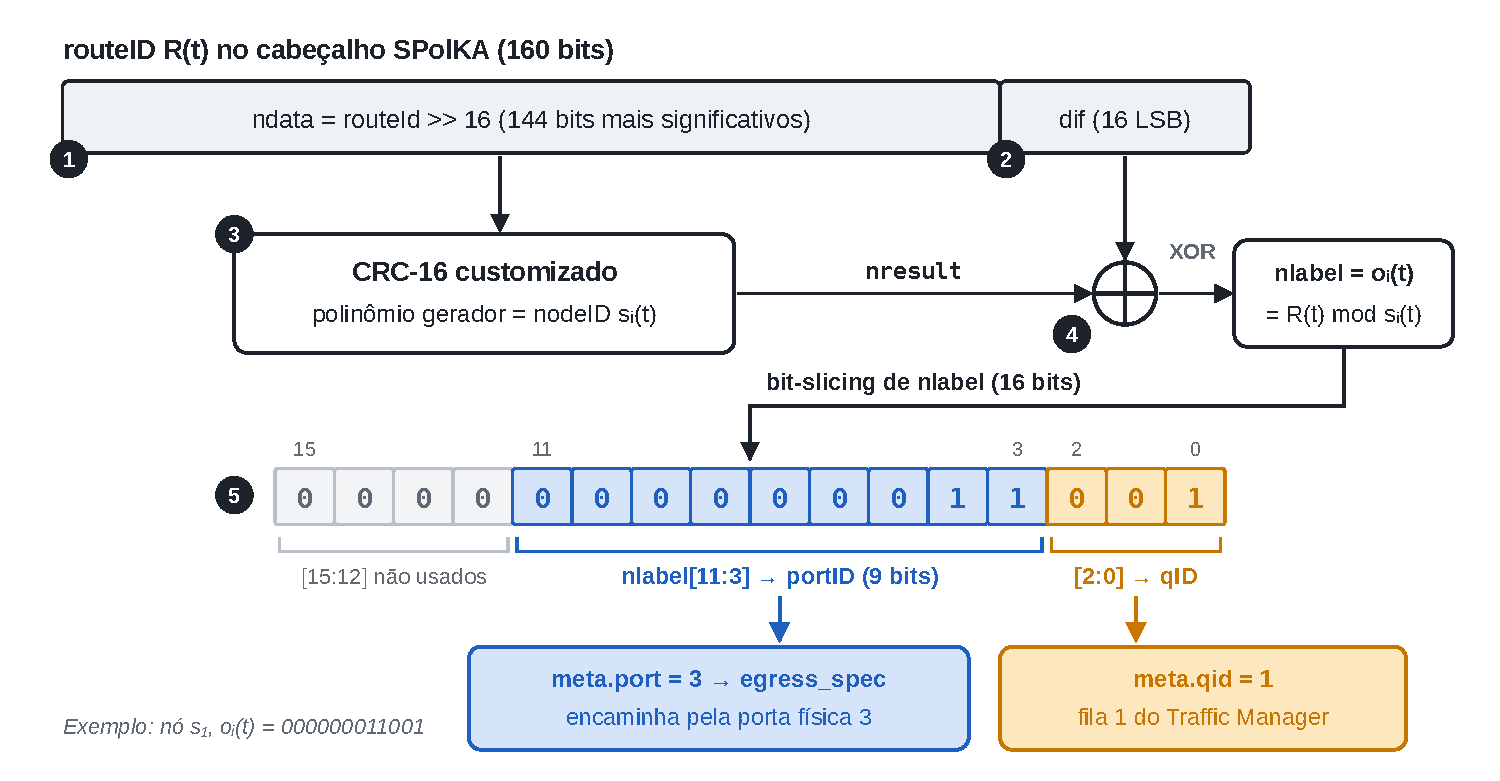
\includegraphics[width=\textwidth]{figuras/fig_a_decodificacao_spolka.pdf}
    \captionsetup{justification=centering}
    \caption{Fluxo de decodificação aritmética e fatiamento de bits (\textit{bit-slicing}) no plano de dados do \nome.}
    \label{fig:decodificacao_spolka}
\end{figure}

O fluxo completo dessa decodificação aritmética no pipeline de ingresso (\textit{Ingress}) de um comutador de núcleo é ilustrado na Figura~\ref{fig:decodificacao_spolka} e detalhado na implementação em linguagem P4 apresentada no Quadro~\ref{quad:codigo_controle}. Inicialmente, o cabeçalho de $160$ bits (\texttt{meta.routeId}) é particionado por meio de um deslocamento lógico de $16$ bits à direita para isolar os $144$ bits mais significativos (\texttt{ndata}, Etapa 1) e de um truncamento direto para extrair os $16$ bits menos significativos (\texttt{dif}, Etapa 2). Em seguida, a unidade de CRC-16 customizada calcula o resto polinomial \texttt{nresult} utilizando o \nodeID\ local como polinômio gerador (Etapa 3), o qual é combinado via operação \texttt{XOR} com \texttt{dif} para reconstituir o polinômio de saída $o_i(t)$ de $16$ bits (\texttt{nlabel}, Etapa 4).

Por fim, aplica-se o fatiamento de bits (\textit{bit-slicing}) sobre \texttt{nlabel} (Etapa 5): considerando uma palavra de controle útil de $12$ bits (com os bits $[15:12]$ reservados para expansões futuras), os $9$ bits intermediários (\texttt{nlabel[11:3]}) definem o identificador da porta física de saída (\portID, suportando até $512$ portas por comutador), enquanto os $3$ bits menos significativos (\texttt{nlabel[2:0]}) especificam o identificador da fila de serviço (\qID, endereçando até $8$ filas distintas por interface). No exemplo da Figura~\ref{fig:decodificacao_spolka}, para o nó $S_1$ com $o_1(t) = 000000011001$, a extração resulta em $\texttt{meta.port} = 3$ e $\texttt{meta.qid} = 1$, direcionando o pacote à fila prioritária $1$ da porta física $3$.

\begin{quadro}[htb]
    \centering
    \caption{Função de cálculo do rótulo SPolKA em linguagem P4}
    \label{quad:codigo_controle}
    \begin{lstlisting}[language=P4]
        action srcRoute_nhop() {
            bit<16> nresult;
    
            // 1. Extração dos 144 bits mais significativos do routeId por deslocamento à direita
            bit<160> ndata = meta.routeId >> 16;
            
            // 2. Truncamento direto para obtenção dos 16 bits menos significativos (termo independente)
            bit<16> dif = (bit<16>)meta.routeId;
    
            // 3. Cálculo do resto da divisão polinomial em GF(2) via unidade de CRC-16 customizado,
            // utilizando constantes literais para otimizar a alocação de registradores
            hash(nresult,
                 HashAlgorithm.crc16_custom,
                 16w0,           // Valor base (offset) nulo
                 {ndata}, 
                 64w8589934592); // Limite superior do domínio de saída (2^33)
    
            // 4. Composição do polinômio de saída o_i(t) via adição modular (XOR)
            bit<16> nlabel = nresult ^ dif;
    
            // 5. Fatiamento de bits (bit-slicing) para decodificação simultânea de encaminhamento e QoS:
            meta.port = (bit<9>)nlabel[11:3]; // Bits [11:3] determinam o identificador da porta de saída (portID)
            meta.qid  = (bit<3>)nlabel[2:0];  // Bits [2:0] especificam o identificador da fila de serviço (qID)
        }
    \end{lstlisting}
    \fonte{Elaborado pelo autor (2026), adaptado de \textcite{nerds_polka}.}
\end{quadro}

% ==============================================================================
\section{Escalonamento Programável e Gerenciamento de Tráfego}
\label{sec:traffic_manager}

A decodificação simultânea do \portID\ e do \qID\ no pipeline de ingresso somente se traduz em isolamento efetivo de QoS quando acoplada a um mecanismo de enfileiramento capaz de impor garantias de largura de banda e evitar a inanição (\textit{starvation}) de fluxos menos prioritários. Enquanto switches de hardware comerciais (como a família Intel Tofino) dispõem de gerenciadores de tráfego nativos configuráveis com algoritmos ponderados, e sistemas operacionais como o Linux oferecem disciplinas de enfileiramento nativas no subsistema \textit{Traffic Control} (\texttt{tc}), ambientes de emulação programável como o \textit{Behavioral Model version 2} (BMv2) implementam originalmente apenas escalonamento por prioridade estrita, no qual filas de menor precedência podem ser completamente bloqueadas sob condições de saturação.

Para superar essa limitação do escalonador nativo do BMv2 e alinhar o comportamento do plano de dados ao requisito \textbf{RF04}, a arquitetura do \nome\ integra um Gerenciador de Tráfego (\textit{Traffic Manager} -- TM) programável acoplado ao final do pipeline de \textit{Ingress}, conforme ilustrado na Figura~\ref{fig:traffic_manager}. Essa solução baseia-se na implementação de referência de escalonadores baseados em classificação em P4 proposta por \textcite{Elbediwy2025}, cujo código-fonte original, por ter sido concebido especificamente para o cenário de avaliação de seu próprio laboratório, apresentava acoplamento rígido às estruturas de cabeçalho e às condições experimentais daquele ambiente. No âmbito deste trabalho, o código em C++ da extensão externa (\textit{extern} \texttt{my\_scheduler}) foi refatorado e generalizado para operar de forma agnóstica aos protocolos encapsulados, permitindo que o algoritmo \textit{Weighted Deficit Round-Robin} (WDRR) seja aplicado a qualquer fluxo de tráfego interceptado após a execução da ação \texttt{srcRoute\_nhop()}.

\begin{figure}[!htb]
    \centering
    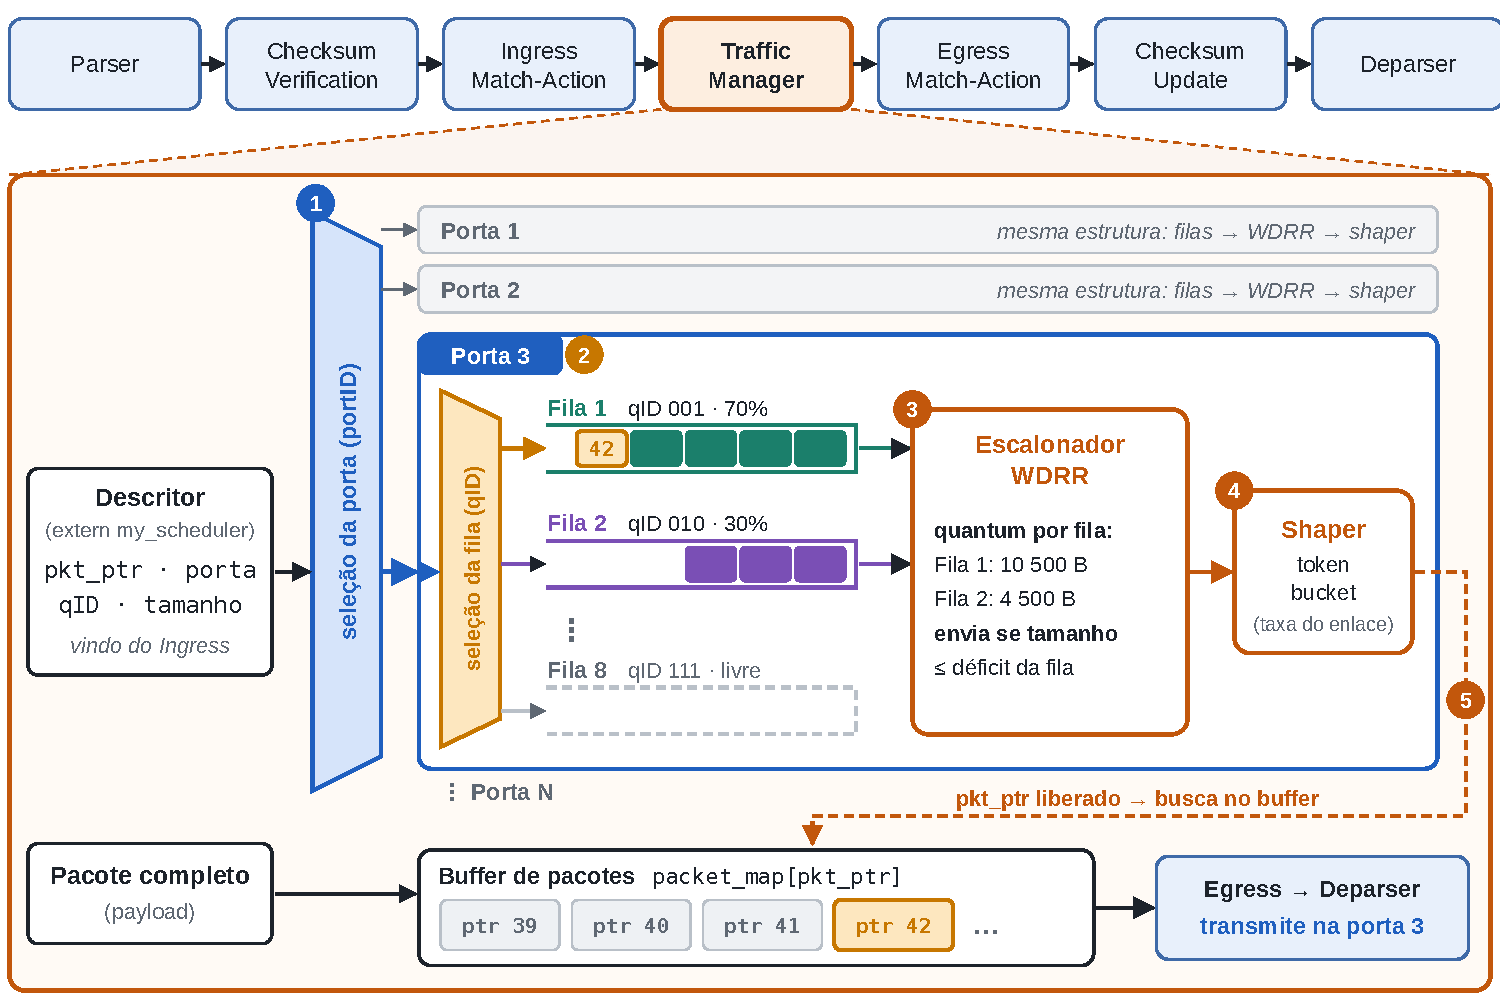
\includegraphics[width=\textwidth]{figuras/fig_b_traffic_manager.pdf}
    \captionsetup{justification=centering}
    \caption{Arquitetura interna do Gerenciador de Tráfego (\textit{Traffic Manager}) programável com escalonamento WDRR e \textit{shaping} por interface.}
    \label{fig:traffic_manager}
\end{figure}

O ciclo de enfileiramento e transmissão no \textit{Traffic Manager} ocorre em cinco etapas coordenadas, destacadas na Figura~\ref{fig:traffic_manager}:
\begin{enumerate}
    \item \textbf{Transferência do Descritor e Armazenamento em Buffer:} Ao concluir o processamento de \textit{Ingress}, o pacote completo (\textit{payload} e cabeçalhos) é armazenado em um buffer compartilhado indexado por um ponteiro único (\texttt{packet\_map[pkt\_ptr]}), enquanto um descritor compacto contendo o ponteiro (\texttt{pkt\_ptr}), a porta de destino (\texttt{portID}), o identificador da fila (\texttt{qID}) e o tamanho do quadro em bytes é repassado ao módulo escalonador.
    \item \textbf{Demultiplexação por Porta e Fila:} Com base no par $(\texttt{portID}, \texttt{qID})$ decodificado a partir do \routeID, o descritor é inserido na estrutura de filas correspondente à interface física de saída (e.g., Porta $3$, Fila $1$ para \texttt{qID = 001} ou Fila $2$ para \texttt{qID = 010}). Cada interface física mantém até $8$ filas lógicas isoladas, suportando tanto fatias com reservas garantidas quanto fatias de melhor esforço (\texttt{qID = 111}).
    \item \textbf{Escalonamento Ponderado via WDRR:} Para arbitrar a ordem de serviço entre as filas ativas de uma mesma porta sem incorrer em inanição, emprega-se o algoritmo \textit{Weighted Deficit Round-Robin} (WDRR). A cada rodada, cada fila não vazia recebe um crédito (\textit{quantum}) em bytes proporcional ao peso da fatia configurada (por exemplo, $10.500\text{ B}$ para a Fila $1$ com reserva de $70\%$ e $4.500\text{ B}$ para a Fila $2$ com reserva de $30\%$). Um pacote somente é desenfileirado se o seu tamanho em bytes for inferior ou igual ao déficit acumulado da respectiva fila; caso contrário, o saldo remanescente é preservado para a rodada subsequente. Além de assegurar o isolamento estrito sob congestionamento, o WDRR permite que uma fatia utilize a banda ociosa de filas inativas, maximizando a eficiência estatística do enlace.
    \item \textbf{Modelagem de Taxa (\textit{Shaping}):} Os descritores selecionados pelo escalonador WDRR passam por um regulador baseado em balde de fichas (\textit{token bucket shaper}), responsável por limitar a taxa de transmissão agregada à capacidade nominal do enlace físico e absorver micro-rajadas de tráfego.
    \item \textbf{Recuperação e Transmissão no Egresso:} Uma vez autorizado pelo \textit{shaper}, o descritor libera o ponteiro \texttt{pkt\_ptr}, permitindo que o pacote original seja recuperado do \texttt{packet\_map}, processado pelo pipeline de \textit{Egress} e pelo \textit{Deparser}, e finalmente transmitido pela interface física de saída.
\end{enumerate}

% ==============================================================================
\section{Reconfiguração Dinâmica e Migração Ágil de Fatias}
\label{sec:migracao_agil}

% Uma das principais vantagens arquiteturais do \nome\ frente aos modelos tradicionais de engenharia de tráfego e fatiamento (tais como MPLS-TE, RSVP-TE ou DiffServ acoplado a roteamento hop-by-hop) reside na agilidade de reconfiguração e na ausência de tempo de convergência no núcleo da rede.

% Em cenários operacionais dinâmicos --- como a chegada repentina de tráfego concorrente em um enlace compartilhado, a degradação de métricas de latência ou a necessidade de promover uma fatia para uma classe de serviço superior ---, a modificação das garantias de QoS no \nome\

Como os comutadores de núcleo não mantêm estados por fluxo nem tabelas de mapeamento de fatias, a transição ocorre de maneira atômica e instantânea no plano de dados, sem perda de pacotes por inconsistência transitória de tabelas e sem sobrecarga de sinalização no plano de controle.

Para validar empiricamente os requisitos levantados e comprovar a eficácia da arquitetura \nome\ sob condições controladas e realistas, foram desenvolvidos dois protótipos complementares: (i) um ambiente emulado baseado em P4/BMv2, estendido com o gerenciador de tráfego programável com escalonamento ponderado (WDRR); e (ii) uma topologia virtualizada em \textit{Containerlab} sobre contêineres Ubuntu 24.04, na qual o processamento de pacotes do \nome\ é executado em eBPF/XDP integrado ao subsistema nativo de controle de tráfego (\texttt{tc}) do \textit{kernel} Linux. O Capítulo~\ref{chap:prototipos} detalha a implementação técnica desses protótipos --- abrangendo a programação dos planos de dados, a configuração dos escalonadores e a orquestração do plano de controle ---, bem como apresenta a metodologia experimental e a análise dos resultados obtidos em termos de isolamento de largura de banda, latência e agilidade na migração de fluxos.